\documentclass[9pt,twocolumn,twoside]{../../styles/osajnl}
\usepackage{fancyvrb}
\journal{i524} 

\title{Apache Lucene}

\author[1,*, +]{Roy Choudhury, Sabyasachi}

\affil[1]{School of Informatics and Computing, Bloomington, IN 47408, U.S.A.}

\affil[*]{Corresponding authors: sabyroyc@indiana.edu}

\affil[+]{HID - S17-IO-3015}

\dates{project-000, \today}

\ociscodes{Search Engine Library, Lucene}

% replace this with your url in github/gitlab
\doi{\url{https://github.com/sabyasachi087/sp17-i524/tree/master/paper1/S17-IO-3015/report.pdf}}


\begin{abstract}
Apache Lucene is an information retrieval or text searching library, written 
entirely in Java. The purpose is to add boilerplate codes of any search engine,
ready for use and configurable , so that the application can focus on the core
business. On this paper we will walk through the architecture and see the pros
and cons of the library.
\newline
\end{abstract}

\setboolean{displaycopyright}{true}

\begin{document}

\maketitle

\section{Introduction}

Apache Lucene is a search library that enables search facility to any 
application. Although it was initially written in Java but is now available
in other languages too chiefly C-Sharp, c/c++ , Python etc. It is an active
open source project and under Apache License. Lucene is just a search library 
and cannot handle other related operations like crawling, document filtering , 
administration etc. We will get to them individually later in this document.

\subsection{General Concepts}
\emph{Information Overload}  means, difficulty that one can have in making 
decisions, because of the presence of too much of information. In another 
words, "Information Overload" can occur if the rate of feed/input into a 
system exceeds its processing capabilities. Imagine the situation of current 
world. We are living in the world where data has reached volume of zeta bytes.
To extract some insight , first step is to collect all related data. This is 
known as \emph{Information Retrieval (IR)} \cite{wiki-ir}. IR is the task of 
collecting relevant information from collection of data resources scattered 
across devices. 

\section{Search Engine}
Google has set some base expectations for search engines, which if not 
available can cause dissatisfaction for the users. For example spell checker 
and response time of <= 1 second. Lucene should be able to met those 
expectations or else its not worth. But Lucene is not a full fledged search 
engine rather its a tool kit to achieve so. We will be using Web search engine
as an use case to explain terminologies of a search engine. 

Module  : Raw Content -> Gather Data -> Analyse -> Index ->  Query Support 
UseCase : User query -> Search Engine -> Build Query -> Extract Information 
from indexed data
\subsection{Module}
\begin{itemize}

\item Raw Content : For Google, contents are web pages and their urls. Google 
uses crawler to download these information. Crawler is bot or a program that
 systematically searches World Wide Web for the purpose of web indexing.

\item Gather Data : The information from the crawler will be persisted. 
Databases are preferred options to store the information. Plain text file 
can be used as well for this step.

\item Analyse : In this step meta information from the existing data is 
extracted. For an example , say we have a page from url 
"http://www.worldwildlife.org/species/tiger". By analysing the content within 
the page we found it contains world tiger population, their habitats and 
mating seasons, so on and so forth. These information can be compiled and kept 
separately to identify them on aforesaid information. These are known as 
keywords or tags.

\item Indexing : The meta information extracted from the document has to be 
mapped and should be readily available on query. These tags or keywords 
are generally mapped to one or more documents or web page. For example 
the keyword \textit {`tiger count`} can map to both \textit{WorldWildLife} 
and \textit{NatGeo}. 

\item Query Support : This is where queries are parsed and executed to fetch 
the matching results. It includes a parser to make the query which are mostly
human readable format are converted to a format which can be used by the 
program to fetch results.
\end{itemize}

\subsection{UseCase}
\begin{itemize}
\item User Query : From Google perspective this is where user enters the 
search query. This is the entry point for any search application to 
initiate a search.

\item Search Engine :  Engine is the core search program. It is responsible 
for taking the input, process it and return the result.

\item Build Query : Engine will parse the query and build the command requires 
to get the result. 

\item Extract Information : This is the final step where the built query is 
passed into the Query support module and renders the result on to the page. 
\end{itemize}

\section{Architecture}
Figure 1 explains a basic architecture of Lucene

\begin{figure}[htbp]
\centering
\fbox{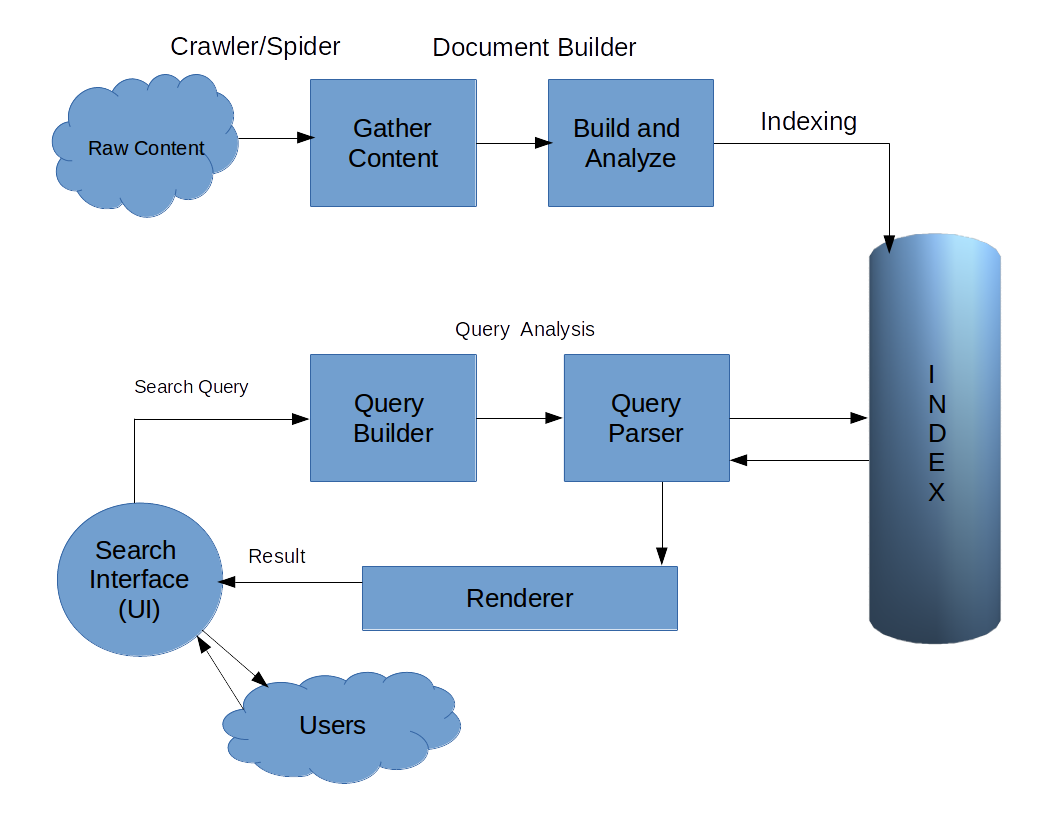
\includegraphics[width=\linewidth]{images/Apache_Lucene_Architecure.png}}
\caption{Apache Lucene Architecture.}
\label{fig:lucene-data-flow}
\end{figure}

Lucene library is compact and does not have any external dependencies. 
Fig 1 \cite{lucene-book} shows process flow of Lucene. On a high level , data 
collected from different sources are analyzed and converted into smaller 
chunks. These are known as documents. Documents are text entries and from these 
text entries Lucene performs indexing and store it in local disk for future 
reference. The next step is to handle the search query from users. Lucene has 
a query parser to understand the query and search the index for the correct or 
relevant match. If found, returns the document back.

\section{Lucene Components}

\subsection{Document Analysis and Indexing}
Data or contents which are available in different format and location needs to be gathered. This process is typically done by a crawler/spider. Core Lucene does not have these capabilities and can be considered to be a pre-requisite for Lucene to implement.Two of the crawler that are build on Lucene are Solr \cite{www-solr} and Nutch \cite{www-nutch}. Once the data is collected , document has to be constructed from the contents. The design of constructing documents has to be decided by the user and implemented within Lucene. Lucene provides an API for building documents but logic has to be provided by the implementation layer. Lucene also does not provide any API for document filtering. Tika , which is built on Lucene, can be used for this purpose. But we cannot index the document yet. We cannot index the raw content within the document directly. Before that , we need to break the content into smaller chunks known as tokens. Each token is map to a "word". Analysis includes handling compound words, spell check, typo correction injection of synonyms, etc. Lucene has built in support of list of error analyzers which gives a fine grain control over analysis. Once tokenization is done , now its time for indexing. Lucene takes care all of the need to cater this step. An API has been provide for this purpose, but has to be implemented carefully as the searching will solely depend upon how well the indexing has been done.


\subsection{Searching}
Searching is the process of looking up within the index to extract the most relevant (matching) documents. It is based on two metrics i.e. \textit{Precision} and \textit{Recall}. Recall measures how well the system finds the relevant documents and Precision measures the filtering out the irrelevant one. Lucene offers benchmarking technique for measuring these matrices. User Interface (UI) is equally important for a search application as that is what the end user is going to use. Lucene does not provide any UI support. When user inputs the search query the first step is to build the query. User inputs are human readable and need further processing before it can be used within the application. Lucene provides a powerful parser for this job known as QueryParser. Even in its default state it does the job but often needs extension as per some advance requirements. Finally hitting the search query to index. All of it is catered by Lucene and also provide option for extension. It finds the result and returns all relevant document objects. Its the responsibility of the UI to render the results correctly.

\section{Advance Usages}
Lucene has some advance feature for administration and analytics. For example Lucene allows to configure the RAM buffer size , re-indexing ,commit and purge scheduler. It allows some fault tolerance mechanism in case a newly added document failed to index. Related to analytics it also provides some meta information regarding the search queries it receives and the results it renders. For example which kind of query are run , query hitting lowest relevance , query having no results and so on. One big problem within the list of advance usages that Lucene does not support is "Scaling". Scaling in terms of both through put and processing speed. In a clustered environment this is quiet an important part as data and resource all are distributed. But both Solr and Nutch provides data partitioning and sharding to achieve higher throughput if not speed. Elastic search is another option which is based upon Lucene and provides distributed computing. Elasticsearch is based on lucene and provides full text search engine with an HTTP based interface (REST Services) and schema free JSON documents. 


\section{Conclusion}
Lucene is the standard library for search applications. It can be compared with 'C' (language) of computing which is small and powerful but requires much more effort to build an entire application. Lucene is just a library which sits at the core of the functionality but it needs much more than that to build an application. Elastic Search , Solr and Nutch which are based on Lucene are preferred tools in terms of building enterprise level search engines. 

\section{Reading Sources}

\begin{itemize}
\item Lucene In Action \cite{lucene-book} provides a startup guide to
learn, build and implement search engines based on Lucene 
\item Lucene at tutorial point \cite{www-lucene-tp} provides introduction
 to Lucene Library.
\end{itemize}



\section*{Acknowledgements}

Thanking Prof. Gregor von Laszewski for his technical help and support.


% Bibliography

\bibliography{references}

\end{document}
